\documentclass[a4paper, twoside, 10pt]{article}

\usepackage[utf8]{inputenc}
\usepackage[naustrian]{babel}
\usepackage[T1]{fontenc}

% "jeder Seitenrand soll 18mm betragen und Kopf- und Fusszeilen inkludieren" interpretiere ich so, dass kopf- und fusszeile
% teil des seitenrandes sind und somit nicht mit includehead/foot teil des bodys gemacht werden sollen
\usepackage[a4paper, margin=18mm, headsep=11mm, footskip=11mm]{geometry}

\usepackage{graphicx}
\usepackage{hyperref}
\usepackage[skip=1.05ex]{parskip}

\usepackage{lipsum} % filler text

\usepackage{fancyhdr}
\fancyhf{} % reset header/footer
\pagestyle{fancy}

% ich ignoriere hier "jede seite muss die gleiche formatierung von kopf- und fusszeilen haben"; innen- und aussenseite haben 
% natuerlich unterschiedliche formatierungen, der angabe folgend
\lhead[\footnotesize{\nouppercase{\leftmark}}]{\footnotesize{Seite \thepage}}
\rhead[\footnotesize{Seite \thepage}]{\footnotesize{\nouppercase{\leftmark}}}
\lfoot[]{\footnotesize{\copyright\ Laurenz Weixlbaumer, k11804751, \today}}
\rfoot[\footnotesize{\copyright\ Laurenz Weixlbaumer, k11804751, \today}]{}

\renewcommand{\headrulewidth}{.75pt}
\renewcommand{\footrulewidth}{.75pt}

\begin{document}

\section{Einführung}

F\"ur Links wird das Paket \texttt{hyperref} \cite{hyperref-doc} verwendet.

\lipsum

\section{Allgemeine Relativit\"atstheorie}

\lipsum

\subsection{Quantenmechanik}

\begin{figure}[htp]
    \centering
    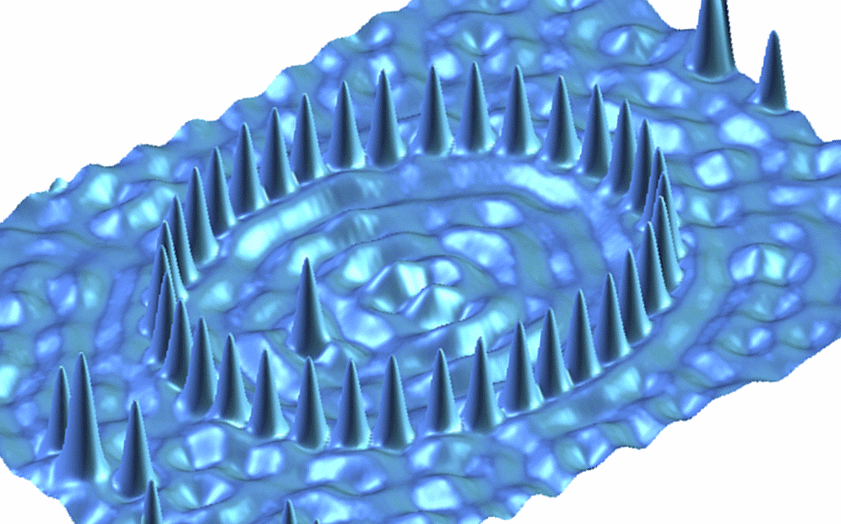
\includegraphics[width=0.5\textwidth]{fig/co-ellipse.png}
    \caption{Die Quantenmechanik sichtbar gemacht: Rastertunnelmikroskopaufnahme von Kobaltatomen auf einer Kupferoberfläche. Das Messverfahren nutzt Effekte, die erst durch die Quantenmechanik erklärt werden können. Auch die Interpretation der beobachteten Strukturen beruht auf Konzepten der Quantenmechanik. \cite{fig-co-ellipse}}
    \label{fig:co-ellipse}
\end{figure}

\lipsum

\subsection{Kosmologie}

\begin{figure}[htp]
    \centering
    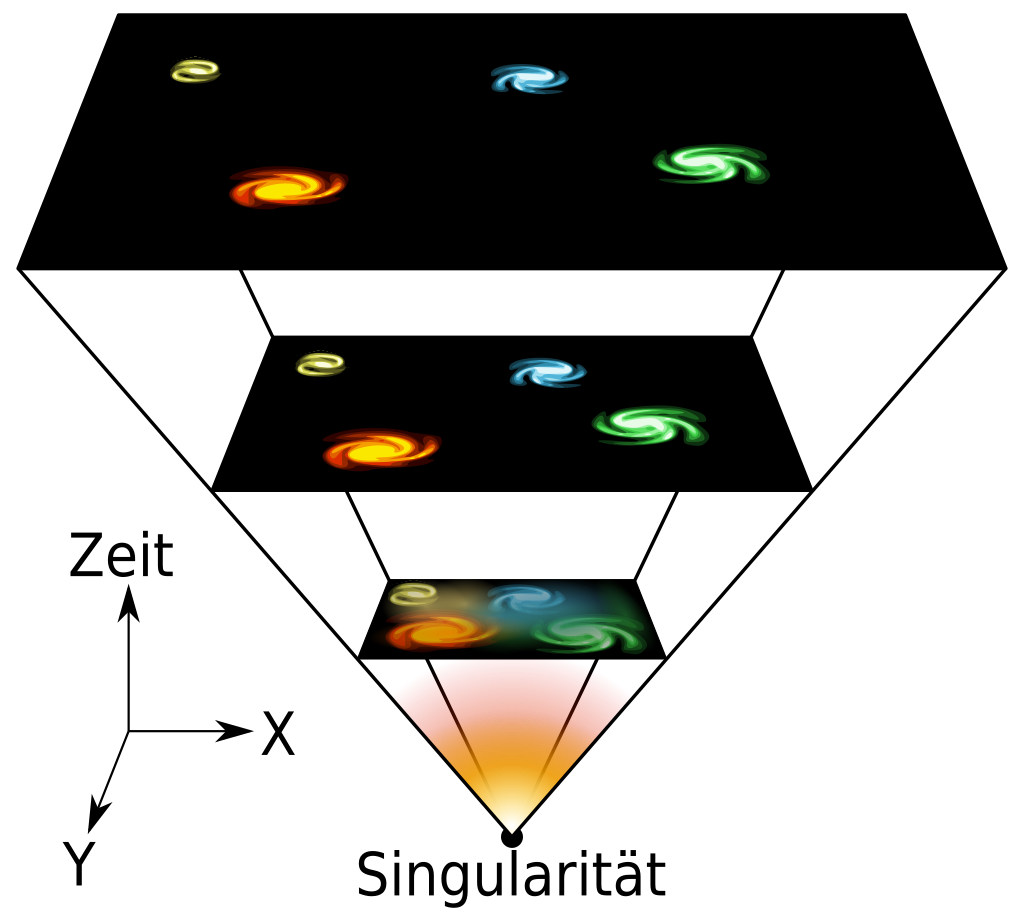
\includegraphics[width=0.5\textwidth]{fig/universe-expansion-de.png}
    \caption{Entstehung des Universums beim Urknall. \cite{fig-universe-expansion}}
    \label{fig:urknall}
\end{figure}

\lipsum

\listoffigures

\begin{thebibliography}{9}
    \bibitem{fig-co-ellipse}
    \url{http://www.nist.gov/cnst/epg/atom_manipulation_stm.cfm}

    \bibitem{fig-universe-expansion}
    \url{https://commons.wikimedia.org/wiki/File:Universe-expansion-de.png}

    \bibitem{hyperref-doc}
    \url{https://www.ctan.org/pkg/hyperref}
\end{thebibliography}

\end{document}
